% !TEX root = ../intro-stellar-physics.tex

Hot air rises, as a glider pilot or hawk can tell you. The fluid velocities in question are very subsonic, so we have hydrostatic equilibrium to excellent approximation. But the fluid motions make an enormous difference for heat transport! This state of fluid motions induced by a temperature gradient is known as \emph{convection}. You can perform the following demonstration of the onset of convection.  Brew tea, and pour the hot tea into a saucepan that is on an unlit burner.  Use a straw with your thumb over the top to insert a layer of cold milk under the warm tea in the saucepan.  The temperature difference between the tea and milk will inhibit their mixing. Light the burner, and watch for the development of convection---you will know it when you see it.

\begin{figure}[htbp]
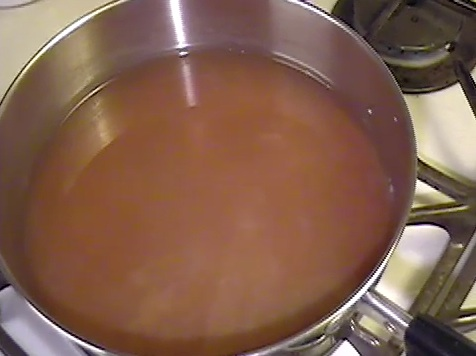
\includegraphics[width=0.5\linewidth]{convection-1}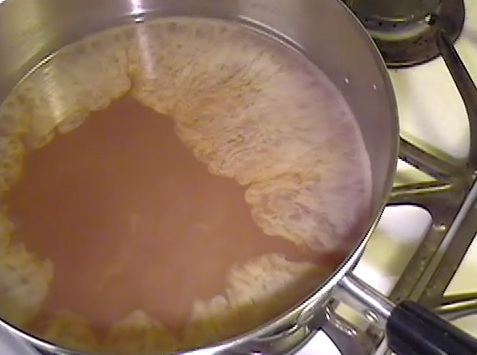
\includegraphics[width=0.5\linewidth]{convection-2}
\caption{Onset of convection in a tea-milk mixture.\label{f.tea}}
\end{figure}

\section{Criteria for onset of convection}\label{s.convection-onset}

To understand this process, let's consider a fluid in planar geometry and hydrostatic equilibrium,
\begin{equation}
\frac{\dif P}{\dif r} = -\rho g.
\end{equation}
Now, imagine moving a blob of fluid upwards from $r$ to $r+h$.  We move the blob slowly enough that it is in hydrostatic equilibrium with its new surroundings, $P_{b}(r+h) = P(r+h)$, where the subscript $b$ refers to ``blob.'' We do move the blob quickly enough, however,  that it does not remain in \emph{thermal} equilibrium with its surroundings; that is, we move the blob \emph{adiabatically}.  The entropy of the blob is therefore constant, 
$S_{b}(r+h) = S_{b}(r) = S(r)$, and is therefore not, in general, equal to the entropy of the surrounding gas at $r+h$: $S_{b}(r+h)  \neq S(r+h)$.  

As the blob rises, it displaces some of the surrounding fluid. Archimedes tells us that if the displaced fluid is less massive than the blob, then the blob will sink.  We can rephrase this in terms of the volume occupied by a unit mass of fluid $V$: if the volume occupied by the blob is less than the volume of an equal mass of background, then the blob will sink. Translating this into an equation: if
\begin{eqnarray}
\lefteqn{V[P(r+h),S(r+h)] - V_{b}[P_{b}(r+h),S_{b}(r+h)] =}\nonumber\\
&&  V[P(r+h),S(r+h)] - V[P(r+h),S(r)] > 0
\label{e.archimedes}
\end{eqnarray}
then the blob will sink. If condition (\ref{e.archimedes}) is violated, the blob will continue to rise, and the system is unstable to convection.  
Figure~\ref{f.convective-schematic} has a cartoon of this process.

\begin{marginfigure}
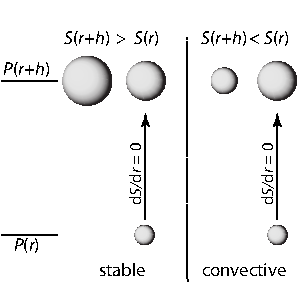
\includegraphics[width=\textwidth]{convective}
\caption[Illustration of criteria for convective instability.]{\label{f.convective-schematic}Illustration of criteria for convective instability.  On the left, raising a blob a distance $h$ adiabatically and in pressure balance with its surrounding results in a higher density $V_{b} < V$.  This is stable: the blob will sink back.  On the right, the blob is less dense and hence buoyant: it will continue to rise.}
\end{marginfigure}

Taking $h$ to be an infinitesimal displacement and expanding the left-hand side of equation~(\ref{e.archimedes}) gives us a local condition for stability:
\begin{equation}\label{e.convective-stability}
V[P(r+h),S(r)] + \tderiv{V}{S}{P}\frac{\dif S}{\dif r} - V[P(r+h),S(r)]  = \tderiv{V}{S}{P}\frac{\dif S}{\dif r} > 0 .
\end{equation}
Noting that
\begin{eqnarray*}
\tderiv{V}{T}{P} &=& \tderiv{V}{S}{P}\tderiv{S}{T}{P}\\
 &=& \frac{C_{P}}{T}\tderiv{V}{S}{P},
 \end{eqnarray*}
 we can rewrite equation~(\ref{e.convective-stability}) as
 \[
 \frac{T}{C_{P}}\tderiv{V}{T}{P}\frac{\dif S}{\dif r} > 0.
 \]
Now, $(\partial V/\partial T)_{P}$ is positive (gas expands on being heated), so our condition for stability is simply
 \begin{equation}\label{e.entropy-condition}
\frac{\dif S}{\dif r} > 0.
\end{equation}
In a convectively stable star, the entropy must increase with radius. if $\dif S/\dif r < 0$, then convection occurs and carries high-entropy material outward, where it will eventually mix with the ambient medium.  As a result, convection drives the entropy gradient toward the marginally stable configuration $\dif S/\dif r = 0$.  If a star is fully convective and mixes efficiently, then the interior of the star lies along an adiabat. 

\newthought{We can derive a condition for convective stability} in terms of the local gradients of temperature and pressure. Writing $S = S[P(r),T(r)]$ we expand equation~(\ref{e.entropy-condition}) to obtain
\begin{equation}\label{e.schwarzschild-1}
\frac{\dif S}{\dif r} = \tderiv{S}{P}{T} \frac{\dif P}{\dif r} + \tderiv{S}{T}{P}\frac{\dif T}{\dif r} .
\end{equation}
Now, $P$ is a monotonically decreasing function of $r$, which means we can use it as a spatial coordinate and write,
\begin{equation}\label{e.TPstar}
\frac{\dif T}{\dif r} = \TPstar \frac{\dif P}{\dif r} .
\end{equation}
Here $\dif T/\dif P|_{\star}$ is the slope of the $T(P)$ relation \emph{for the stellar interior}.  In particular, this is \emph{not} a thermodynamic equality. Substituting equation~(\ref{e.TPstar}) into equation~(\ref{e.schwarzschild-1}), using hydrostatic equilibrium to eliminate $\dif P/\dif r$, and recognizing that $(\partial S/\partial T)_{P} = C_{P}/T$, we obtain
\begin{equation}\label{e.schwarzschild-2}
\frac{\dif S}{\dif r} =  -\rho g\left[\tderiv{S}{P}{T} + \frac{C_{P}}{T} \TPstar \right].
\end{equation}
Finally, we can use the identity (see Appendix~\ref{s.thermo-derivatives})
\begin{equation}
\tderiv{S}{P}{T}\tderiv{T}{S}{P}\tderiv{P}{T}{S} = -1
\end{equation}
to simplify equation~(\ref{e.schwarzschild-2}),
\begin{eqnarray}
\frac{\dif S}{\dif r} &=& -\frac{\rho g}{P}C_{P}\left[\frac{P}{T}\TPstar - \frac{P}{T}\tderiv{T}{P}{S}\right]\nonumber \\
 & = & -\frac{\rho g}{P}C_{P}\left[\nabla - \nablaad\right].
 \label{e.schwarzschild}
\end{eqnarray}
Here we have introduced the shorthand notation $\nabla\equiv \dif \ln T/\dif\ln P|_{\star}$ and $\nablaad \equiv \left(\partial \ln T/\partial\ln P\right)_{S}$.
\emph{A mixture of uniform composition is unstable to convection if the local temperature gradient is steeper than an adiabat, i.e., if $\nabla > \nablaad$.}
